\begin{figure}
    \centering
    \setlength{\resLen}{0.8in}
    \addtolength{\tabcolsep}{-3pt}
    \begin{tabular}{cccc}
        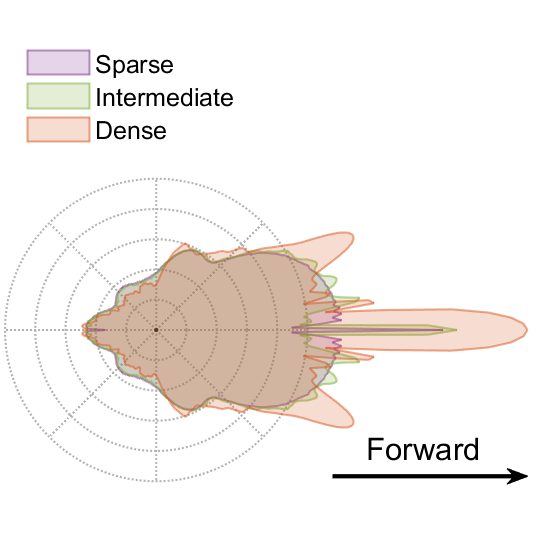
\includegraphics[width=\resLen]{images/pfunc/distance.png} &
        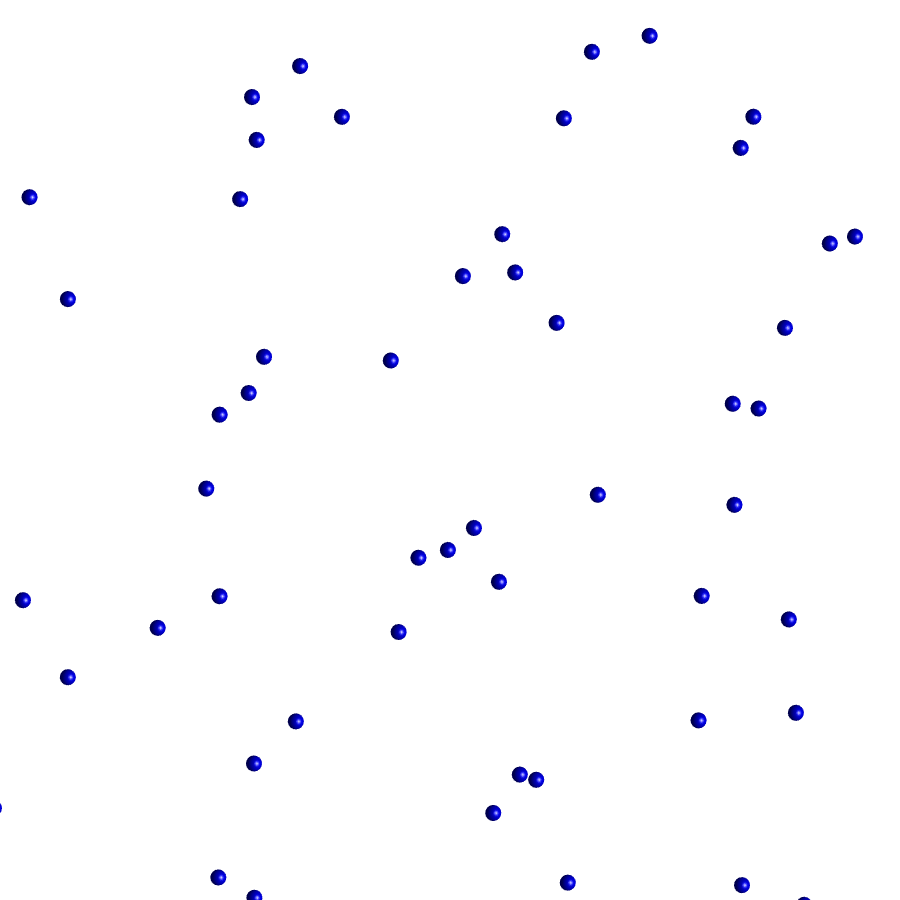
\includegraphics[width=\resLen]{images/particle/validate2_D1_N100_500nm.png} &
        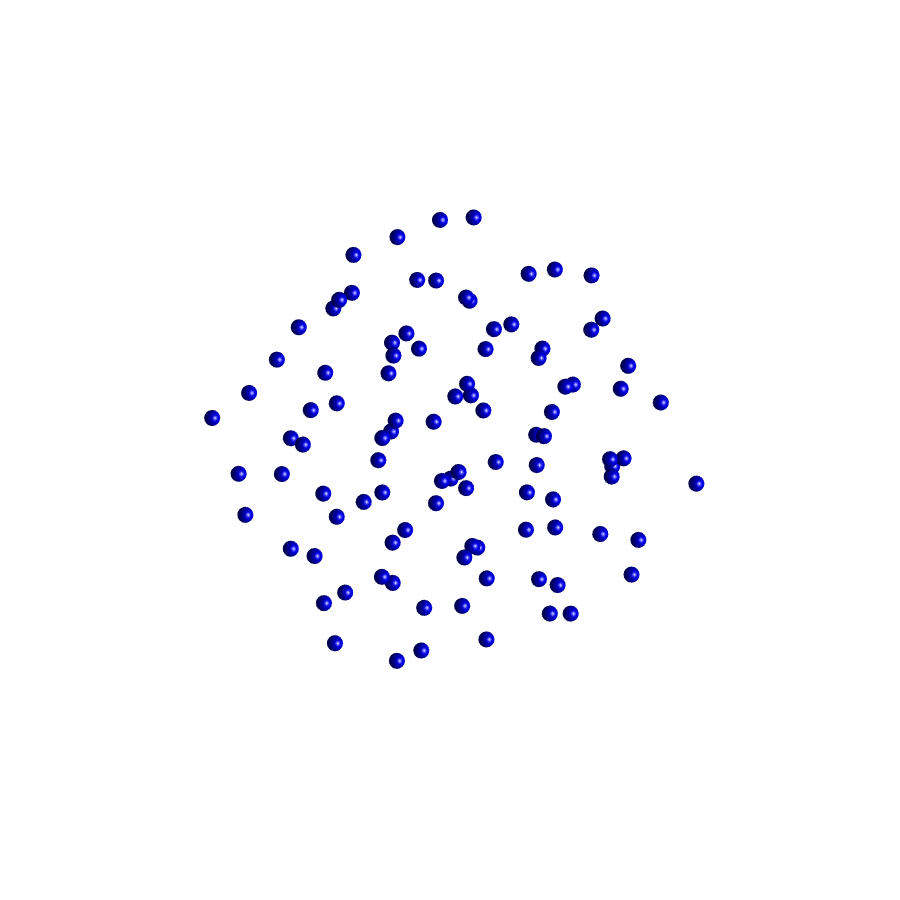
\includegraphics[width=\resLen]{images/particle/validate3_D2_N100_500nm.png} &
        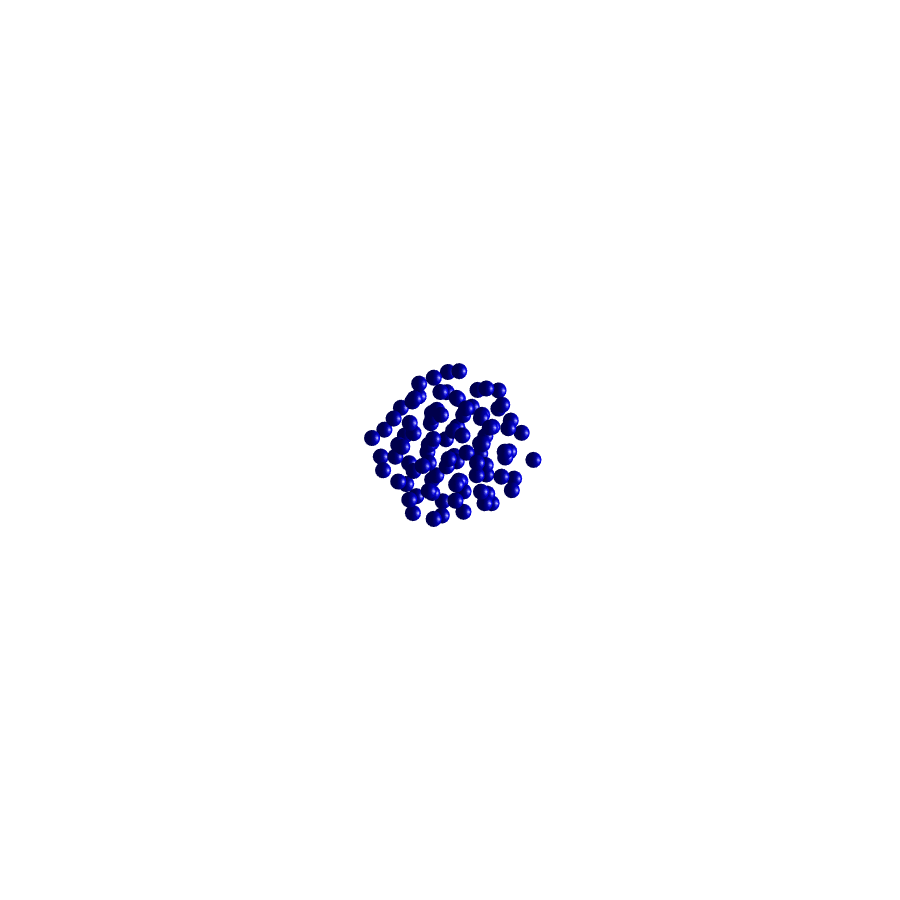
\includegraphics[width=\resLen]{images/particle/validate4_D3_N100_500nm.png} 
        \\
        Phase function & Sparse & Intermediate & Dense
    \end{tabular}
    \caption{\label{fig:sparsity}
       Different distance between particles. Wavelength is 700nm, particle size is 500nm, and 100 particles in a cluster.
    }
\end{figure}

